
\section{Ejercicios de Combinatoria \cite{balakrishnan1995combinatorics}}
% Problemas 1.7, 1.8, 1.29, 1.39, 1.40, 1.77, 1.78, 1.87
% 5 ejemplos de muestras ordenadas

\subsection{Problema 1.7}
Demostrar que un número palindrómico (decimal) de longitud par es divisible por
11.

\textbf{Solución}

La prueba inductiva explota el hecho de que cuando se quitan el primer y el
último carácter de un palíndromo, queda un palíndromo. Así, sea $N$ un número
palindrómico de longitud $2k$. Si $k = 1$, el teorema obviamente se cumple. Si
$k \geq 2$, tenemos

\begin{center}
$ N = a_{2k-1} 10^{2k-1} + a_{2k-2} 10^{2k-2} + ... + a_{k} 10^{k} + ... +
a_{2k-2} 10^{1} + a_{2k-1} 10^{0} $
\end{center}

\begin{center}
$ = a_{2k-1}(10^{2k}+10^0) + (a_{2k-2}10^{2k-2}+...+ a_{2k-2}10^{1}) $
\end{center}

\begin{center}
$ \equiv a_{2k-1} P + Q$
\end{center}

Donde:

\begin{center}
$P = \underbrace{100...001}_{\text{longitud } 2k} =
\underbrace{9090...9091}_{\text{longitud } 2k-2}$
\end{center}

y ya sea $Q=0$ (divisible por 11) o, para algún $1 \leq r \leq k-1$,

$Q = 10^r$ \{palindrome de longitud $ 2(k-r)\} = 10^r\{11R\} $

donde el último paso se sigue de la hipótesis de inducción. Por lo tanto, $N$ es
divisible por 11 y la demostración está completa.

\subsection{Problema 1.8}

En un palíndromo binario, el primer dígito es 1 y cada dígito subsiguiente puede
ser 0 o 1. Cuente los palíndromos binarios de longitud $n$.

\textbf{Solución}

Tenemos $[(n + 1)/2] - 1 = [(n - 1)/2]$ posiciones libres, por lo tanto el número
deseado es:

\begin{center}
$2^{[(n-1)/2]}$
\end{center}

\subsection{Problema 1.29}
Encuentre la probabilidad $p_n$ de que un grupo de $n$ personas reunidas al azar
incluya al menos 2 personas con el mismo cumpleaños (día del año).

\textbf{Solución}

Aquí no tratamos con una muestra de personas, sino con una muestra de
cumpleaños, es decir, números enteros del 1 al 365 inclusivo. Nuestra noción de
probabilidad es:

\begin{center}
$\text{Probabilidad} = \frac{\text{número de muestras favorables}}{\text{Número
total de muestras}}$
\end{center}

En este problema es simple considerar el evento complementario: todos los $n$
cumpleaños son distintos. Este evento es realizado en $P(365,n)$ muestras; y el
total de muestras es $365^n$. Por lo tanto, $1-p_n = P(365,n)/365^n$ o:

\begin{center}
$p_n = 1 - \frac{P(365,n)}{365^n} = 1 -
\frac{(365)(365-1)(365-2)...[365-(n-1)]}{365^n} $
\end{center}

\begin{center}
$= 1-(1 - \frac{1}{365})(1 - \frac{2}{365})...(1 - \frac{n-1}{365})$
\end{center}

Puede verificarse que $p_n \geq 1/2 $ cuando $n>25$.

\subsection{Ejercicio 1.39}
Pruebe que 
\begin{enumerate}
	\item 
    \begin{equation*}
		\Sigma_{r=0}^nC(n,r)=2^n
    \end{equation*}

\textbf{Solución}

\begin{eqnarray*}
	\Sigma_{r=0}^{n} \binom{n}{r}=\Sigma_{r=0}^{n} \binom{n}{r}(1^{n-r})(1^r)=(1+1)^n=2^n
\end{eqnarray*}
	
    \item 
    \begin{equation*}
		\Sigma_{r=0}^n(-1)^rC(n,r)=0
	\end{equation*}

\textbf{Solución}

\begin{eqnarray*}
	\Sigma_{r=0}^{n} (-1)^r \binom{n}{r}=\Sigma_{r=0}^{n} \binom{n}{r}(1^{n-r})(-1^r)=(1-1)^n=0
\end{eqnarray*}

\item
\begin{equation*}
	\Sigma_{r=even}^nC(n,r)=\Sigma_{r=odd}^nC(n,r)=2^{n-1}
\end{equation*}

\textbf{Solución}

\begin{eqnarray*}
	\Sigma_{r=even}^nC(n,r)=\frac{\Sigma_{r=0}^{n} \binom{n}{r}}{2}=\frac{2^n}{2}=2^{n-1}\\
	\Sigma_{r=odd}^nC(n,r)=\frac{\Sigma_{r=0}^{n} \binom{n}{r}}{2}=\frac{2^n}{2}=2^{n-1}
\end{eqnarray*}
	
\end{enumerate}

\subsection{Ejercicio 1.39}
Obtenga nuevamente los resultados del ejercicio 1.39 con argumentos combinatorios.

\textbf{Solución}

\begin{enumerate}
	
\item Si se considera un conjunto de $n$ elementos, se pueden formar $2^n$
subconjuntos (conjunto potencia). El conjunto potencia incluye los subconjuntos
que se pueden formar con r elementos. Así:

\begin{equation*}
	|\mathcal{P}|=2^n=\binom{n}{0}+\binom{n}{1}+...+\binom{n}{n-1}+\binom{n}{n}=\Sigma_{r=0}^{n} \binom{n}{r}
\end{equation*} 

\item Se establece que X tiene tantos subconjuntos con $r$ elementos pares como
$r$ elementos impares.

Caso 1: Esto se cumple si n es impar.
	
Caso 2: Cuando $n$ es par.

Se descompone $X=X'\cup \{j\}$. Donde $j$ es un elemento de $X$\\
	
Ahora $X'$ está compuesto por un n\'umero impar de elementos, por lo que tiene
la misma cantidad de subconjuntos formados con $r$ par ($X_p$) o impar ($X_i$),
pero como se había eliminado un elemento $|X_p|=|X_i|=2^{n-1}$

\end{enumerate}

\subsection{Ejercicio 1.77}

Muestre que en un grupo de n personas, al menos 2 personas conocen al mismo
n\'umero de personas.

\textbf{Solución}

Sea $k$ el n\'umero de personas que no conoce a nadie del grupo

\begin{itemize}
\item Caso $k>1$: Hay m\'as de una persona que no conoce a nadie y entonces se
cumple el enunciado.
	
\item Caso $k=0$: Como no hay persona que no conozca a nadie. Todas las personas
pueden conocer al menos a 1 persona o hasta $n-1$ personas. 
	
Con el principio del palomar (principio de Dirichlet), supongamos que las cajas
(pichoneras) están de acuerdo al n\'umero de personas conocidas. Es decir, que
puede haber hasta $n-1$ pichoneras y que le han preguntado a las $n-1$ personas
a cuántos de los otros conocen. En el caso extremo, uno a uno se ir\'an
colocando en las cajas correspondientes a sus n\'umeros.
	
Cuando le pregunten a la persona $n$, forsozamente tendr\'a que elegir un
n\'umero que alguien m\'as haya elegido y entonces el enunciado se cumple. 
	
\item Caso $k=1$: Se puede despreciar a esa persona que no conoce a nadie y
entonces se hace el an\'alisis para el caso k=0 con un grupo de $n-1$ personas.

\end{itemize}

\subsection{Problema 1.78}

Considera un torneo in el cual cada uno de los $n$ jugadores juega contra cada
uno de los otros jugadores y cada jugador gana al menos 1 juego. Prueba que hay
al menos dos jugadores que tienen el mismo n\'umero de victorias.

El n\'umero de victorias de cada jugador es al menos una y por mucho $n-1$
victorias. Estos $n-1$ n\'umeros corresponde a las pichoneras para acomodar $n$
palomas.

\subsection{Problema 1.87}
Hay 12 computadoras y 8 impresoras l\'aser en una oficina. Encuentra el n\'umero
m\'inimo de conexiones que se tienen que hacer para garantizar que si 8 o menos
computadoras quieren imprimir al mismo tiempo, cada una de ellas ser\'a capaz de
usar una impresora diferente.\\

Suponemos que las impresoras se denotan por $P_{j} (j=1,2,...,8)$ y las
computadoras por $C_{i} (i=1,2,..,12)$.\\

Conectar la primera impresora a las primeras cinco computadoras. Despu\'es
conectar la segunda impresora a las 5 impresoras consecutivas empezando por
$C_{2}$. Despu\'es conectar la tercera impresora con las 5 computadoras
consecutivas empezando por $C_{3}$ y as\'i consecutivamente para generar la
matriz de conexiones.

\begin{table}[h!]
    \centering
	\begin{tabular}{l|lllllllll}
		       &$P_{1}$&$P_{2}$&$P_{3}$ &$P_{4}$&$P_{5}$&$P_{6}$&$P_{7}$&$P_{8}$&\\\hline
		$C_{1}$&  1&  0&  0&   0& 	 0&   0&   0&  0&\\ 
		$C_{2}$&  1&  1&  0&   0& 	 0&   0&   0&  0&\\
		$C_{3}$&  1&  1&  1&   0& 	 0&   0&   0&  0&\\
		$C_{4}$&  1&  1&  1&   1& 	 0&   0&   0&  0&\\
		$C_{5}$&  1&  1&  1&   1& 	 1&   0&   0&  0&\\
		$C_{6}$&  0&  1&  1&   1& 	 1&   1&   0&  0&\\
		$C_{7}$&  0&  0&  1&   1& 	 1&   1&   1&  0&\\
		$C_{8}$&  0&  0&  0&   1& 	 1&   1&   1&  1&\\
		$C_{9}$&  0&  0&  0&   0& 	 1&   1&   1&  1&\\
		$C_{10}$&  0&  0&  0&   0& 	 0&   1&   1&  1&\\
		$C_{11}$&  0&  0&  0&   0& 	 0&   0&   1&  1&\\
		$C_{12}$&  0&  0&  0&   0& 	 0&   0&   0&  1&\\
	\end{tabular}
\end{table}

Sean las 8 computadoras que requieren una impresora $C_{i_{1}}, C_{i_{2}},...,
C_{i_{8}}$ donde $i_{1} <i_{2}<...<i_{8} < $. Si 8 computadoras pueden ser
acomodadas, entonces se puede acomodar cualquier n\'umero m\'as peque\~no. La
observaci\'on crucial es:

\begin{equation}
	s \leq i_{s} \leq s+4   (s=1,2,...,8)
\end{equation}

En efecto, si $i_{s} < s$ existen $s$ enteros positivos menores que $s$ y si
$i_{s} > s+5$, al menos $12-(s+6)+1=7-s$ valores estar\'ian disponibles para los
$8-s$ indices restantes.\\


\section{Ejercicios de Probabilidad \cite{schiller2012probability}}
% Problemas 2.29, 2.30, 2.68 al 2.74

\subsection{Problema 2.29}
Construya el diagrama de árbol para las permutaciones de $\{ a,b,c \}$.

\begin{figure}[h]
	\begin{center}		
	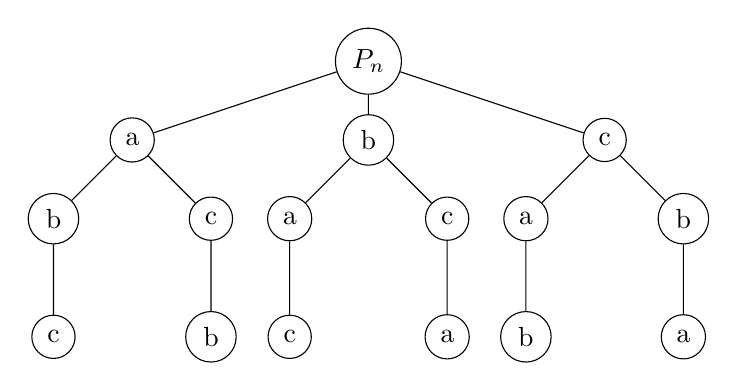
\begin{tikzpicture}[level distance=1cm, level 1/.style={sibling distance=3cm},
		level 2/.style={sibling distance=2cm}, every node/.style={circle, draw,
		align=center} ]
				\centering
				\node[circle,draw]{$P_n$}
		child{node{a} child{node{b} child{node{c}} } child{node{c} child{node{b}}} }
		child{node{b} child{node{a} child{node{c}} } child{node{c} child{node{a}}} }
		child{node{c} child{node{a} child{node{b}} } child{node{b} child{node{a}}} };
			\end{tikzpicture}
		\end{center}
		\caption{Permutaciones para 3 elementos}
		\label{permutaciones_tree}
\end{figure}

\subsection{Problema 2.30}

Una persona tiene tiempo para jugar a la ruleta cinco veces como máximo. En cada
jugada gana o pierde un dólar.

La persona comienza con un dólar y dejará de jugar antes de las cinco veces si
pierde todo su dinero o si gana tres dólares, es decir, si tiene cuatro dólares.
Encuentre el número de formas en que pueden ocurrir las apuestas.


El diagrama de árbol describe la forma en que se pueden realizar
las apuestas. Cada número en el diagrama denota la cantidad de dólares que tiene
el hombre en ese momento. Observe que las apuestas pueden ocurrir de 11 maneras
diferentes. Tenga en cuenta que dejará de apostar antes de que se cumplan los
cinco tiempos en solo tres de los casos.

% Set the overall layout of the tree
\tikzstyle{level 1}=[level distance=1.5cm, sibling distance=3.5cm]
\tikzstyle{level 2}=[level distance=1.5cm, sibling distance=3.5cm]
\tikzstyle{level 3}=[level distance=1.5cm, sibling distance=3cm]
\tikzstyle{level 4}=[level distance=1.0cm, sibling distance=2.5cm]
\tikzstyle{level 5}=[level distance=1.0cm, sibling distance=0.5cm]

% Define styles for bags and leafs
\tikzstyle{bag} = [text width=1em, text centered]
\tikzstyle{end} = [circle, minimum width=0.5pt,fill, inner sep=0pt]

\begin{figure}[h]
    \centering
\begin{tikzpicture}[grow=right, sloped]
    \node[bag] {1}
    child {
        node[bag] {0}
        }
    child {
        node[bag] {2}% This is the first of three "Bag 2"
        child {
                node[bag] {3}
                child{
                        node[bag] {2}
                                                    child {
                             node[bag] {3}
                                                         child {
                             node[bag] {4}
                }
                            child {
                             node[bag] {2}
                }
                }
                            child {
                             node[bag] {1}
                                                         child {
                             node[bag] {2}
                }
                            child {
                             node[bag] {0}
                }
                }
                }
                child{
                        node[bag] {4}
                }
            }
            child {
                node[bag] {1}
                child {
        node[bag] {2}
            child {% Here are three children, hence three end branches
                node[bag] {3}
                            child {
                             node[bag] {2}
                }
                            child {
                             node[bag] {0}
                }
            }
            child {
                node[bag] {1}
                            child {
                             node[bag] {2}
                }
                            child {
                             node[bag] {0}
                }
            }
    }
            }
    };
\end{tikzpicture}
\caption{Diagrama de árbol que describe las formas en las que se pueden realizar
las apuestas.}
\end{figure}

\begin{landscape}

\subsection{Problema 2.68}
Construye el diagrama de árbol para el número de permutaciones de $\{ a,b,c,d
\}$

\begin{figure}[h!]
    \centering
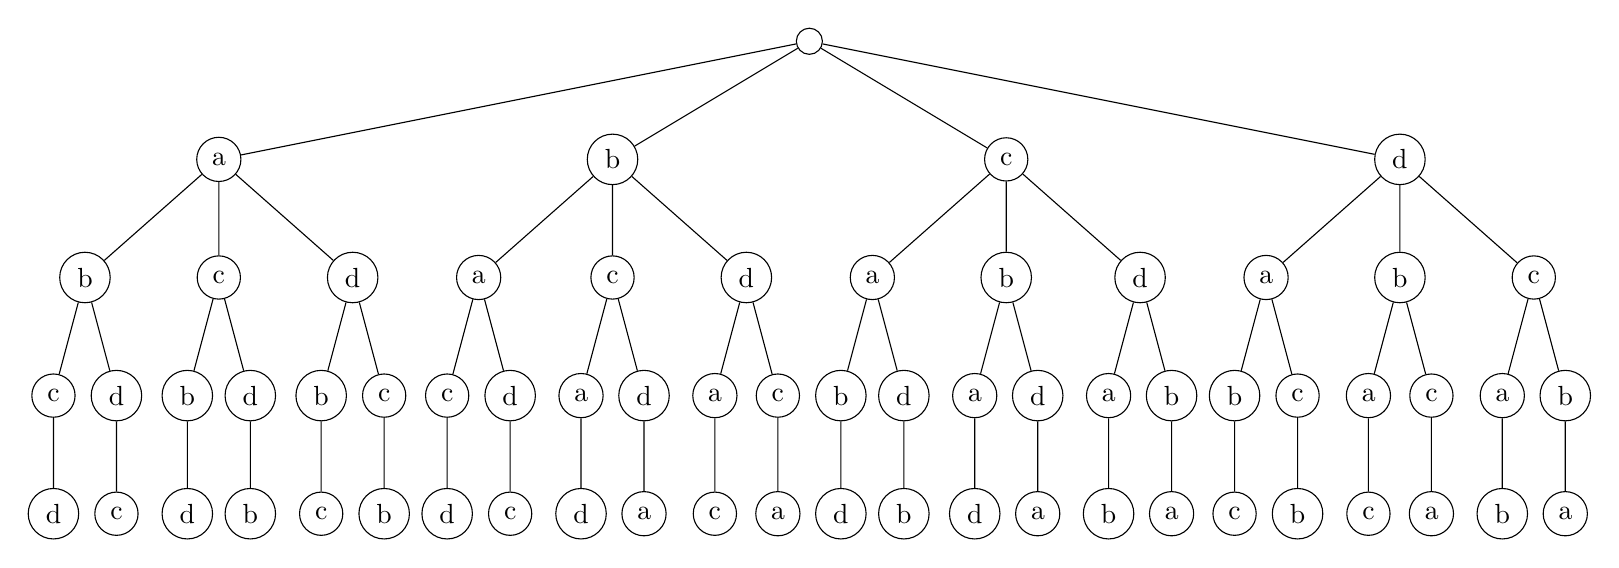
\begin{tikzpicture}[
    auto,
    level 1/.style={sibling distance=50mm},
    level 2/.style={sibling distance=17mm},
    level 3/.style={sibling distance=8mm},
    ]
    \node [circle,draw] (z){}
        child {
            node[circle,draw] (b) {a}
            child { 
                node[circle,draw] (c) {b}
                child {
                    node[circle,draw] (d) {c}
                    child {
                        node[circle,draw] (e) {d}
                    }
                }
                child {
                    node[circle,draw] (d) {d}
                    child {
                        node[circle,draw] (e) {c}
                    }
                }               
            }
             child { 
                node[circle,draw] (c) {c}
                child {
                    node[circle,draw] (d) {b}
                    child {
                        node[circle,draw] (e) {d}
                    }
                }
                child {
                    node[circle,draw] (d) {d}
                    child {
                        node[circle,draw] (e) {b}
                    }
                }               
            } 
            child { 
                node[circle,draw] (c) {d}
                child {
                    node[circle,draw] (d) {b}
                    child {
                        node[circle,draw] (e) {c}
                    }
                }
                child {
                    node[circle,draw] (d) {c}
                    child {
                        node[circle,draw] (e) {b}
                    }
                }               
            }  
        }
        child {
            node[circle,draw] (b) {b}
                        child { 
                node[circle,draw] (c) {a}
                child {
                    node[circle,draw] (d) {c}
                    child {
                        node[circle,draw] (e) {d}
                    }
                }
                child {
                    node[circle,draw] (d) {d}
                    child {
                        node[circle,draw] (e) {c}
                    }
                }               
            }
                       child { 
                node[circle,draw] (c) {c}
                child {
                    node[circle,draw] (d) {a}
                    child {
                        node[circle,draw] (e) {d}
                    }
                }
                child {
                    node[circle,draw] (d) {d}
                    child {
                        node[circle,draw] (e) {a}
                    }
                }               
            }
                       child { 
                node[circle,draw] (c) {d}
                child {
                    node[circle,draw] (d) {a}
                    child {
                        node[circle,draw] (e) {c}
                    }
                }
                child {
                    node[circle,draw] (d) {c}
                    child {
                        node[circle,draw] (e) {a}
                    }
                }               
            }
        }
        child {
            node[circle,draw] (b) {c}
                        child { 
                node[circle,draw] (c) {a}
                child {
                    node[circle,draw] (d) {b}
                    child {
                        node[circle,draw] (e) {d}
                    }
                }
                child {
                    node[circle,draw] (d) {d}
                    child {
                        node[circle,draw] (e) {b}
                    }
                }               
            }
                        child { 
                node[circle,draw] (c) {b}
                child {
                    node[circle,draw] (d) {a}
                    child {
                        node[circle,draw] (e) {d}
                    }
                }
                child {
                    node[circle,draw] (d) {d}
                    child {
                        node[circle,draw] (e) {a}
                    }
                }               
            }
                        child { 
                node[circle,draw] (c) {d}
                child {
                    node[circle,draw] (d) {a}
                    child {
                        node[circle,draw] (e) {b}
                    }
                }
                child {
                    node[circle,draw] (d) {b}
                    child {
                        node[circle,draw] (e) {a}
                    }
                }               
            }
        }
        child {
            node[circle,draw] (b) {d}
                       child { 
                node[circle,draw] (c) {a}
                child {
                    node[circle,draw] (d) {b}
                    child {
                        node[circle,draw] (e) {c}
                    }
                }
                child {
                    node[circle,draw] (d) {c}
                    child {
                        node[circle,draw] (e) {b}
                    }
                }               
            }
                       child { 
                node[circle,draw] (c) {b}
                child {
                    node[circle,draw] (d) {a}
                    child {
                        node[circle,draw] (e) {c}
                    }
                }
                child {
                    node[circle,draw] (d) {c}
                    child {
                        node[circle,draw] (e) {a}
                    }
                }               
            }
                        child { 
                node[circle,draw] (c) {c}
                child {
                    node[circle,draw] (d) {a}
                    child {
                        node[circle,draw] (e) {b}
                    }
                }
                child {
                    node[circle,draw] (d) {b}
                    child {
                        node[circle,draw] (e) {a}
                    }
                }               
            }
        }
        
        ;
\end{tikzpicture}
\caption{Permutaciones para 4 elementos}
\end{figure}


\end{landscape}

% \subsection{Problema 2.69}
% Encontrar el producto de los conjuntos $\{1,2,3\} x \{2,3,4\}$ construyendo el
% diagrama apropiado.
% 
% \subsection{Problema 2.70}
% Los equipos A y B juegan en un torneo de baloncesto. El primer equipo que gana
% dos juegos seguidos o un total de cuatro juegos gana el torneo. Halla el número
% de formas en que puede ocurrir el torneo.



\subsection{Problema 2.71}
Una persona tiene tiempo para jugar a la ruleta cinco veces. Gana o pierde un
dólar en cada jugada. El hombre comienza con dos dólares y dejará de jugar antes
de las cinco veces si pierde todo su dinero o gana tres dólares (es decir, tiene
cinco dólares). Encuentre el número de formas en que puede ocurrir el juego.

% Set the overall layout of the tree
\tikzstyle{level 1}=[level distance=1.5cm, sibling distance=3.5cm]
\tikzstyle{level 2}=[level distance=1.5cm, sibling distance=3.5cm]
\tikzstyle{level 3}=[level distance=1.5cm, sibling distance=3cm]
\tikzstyle{level 4}=[level distance=1.0cm, sibling distance=2.5cm]
\tikzstyle{level 5}=[level distance=1.0cm, sibling distance=0.5cm]

% Define styles for bags and leafs
\tikzstyle{bag} = [text width=1em, text centered]
\tikzstyle{end} = [circle, minimum width=0.5pt,fill, inner sep=0pt]

\begin{figure}[h]
    \centering
\begin{tikzpicture}[grow=right, sloped]
    \node[bag] {2}
    child {
        node[bag] {0}
        }
    child {
        node[bag] {2}% This is the first of three "Bag 2"
        child {
                node[bag] {3}
                child{
                        node[bag] {2}
                                                    child {
                             node[bag] {3}
                                                         child {
                             node[bag] {4}
                }
                            child {
                             node[bag] {2}
                }
                }
                            child {
                             node[bag] {1}
                                                         child {
                             node[bag] {2}
                }
                            child {
                             node[bag] {0}
                }
                }
                }
                child{
                        node[bag] {4}
                }
            }
            child {
                node[bag] {1}
                child {
        node[bag] {2}
            child {% Here are three children, hence three end branches
                node[bag] {3}
                            child {
                             node[bag] {2}
                }
                            child {
                             node[bag] {0}
                }
            }
            child {
                node[bag] {1}
                            child {
                             node[bag] {2}
                }
                            child {
                             node[bag] {0}
                }
            }
    }
            }
    };
\end{tikzpicture}
\caption{Diagrama de árbol que describe las formas en las que se pueden realizar
las apuestas.}
\end{figure}



\subsection{Problema 2.72}
Un hombre está en el origen sobre el eje x y da un paso unitario hacia la
izquierda o hacia la derecha. Se detiene después de 5 pasos o si llega a 3 o -2.
Construya el diagrama de árbol para describir todos los caminos posibles que el
hombre puede recorrer.

\begin{figure}[h!]
	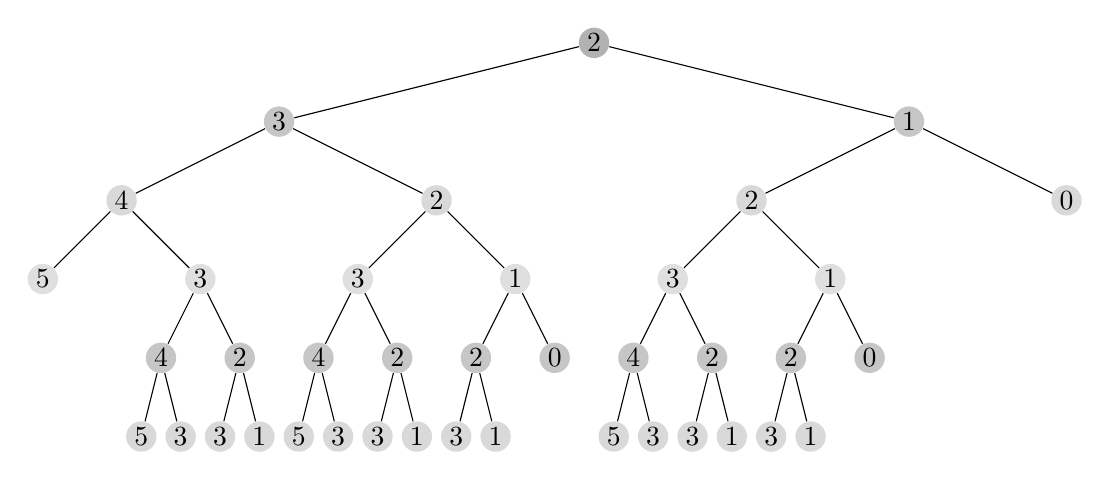
\begin{tikzpicture}
	[level distance=10mm,
	every node/.style={fill=gray!60,circle,inner sep=1pt},
	level 1/.style={sibling distance=80mm,nodes={fill=gray!45}},
	level 2/.style={sibling distance=40mm,nodes={fill=gray!30}},
	level 3/.style={sibling distance=20mm,nodes={fill=gray!25}},
	level 4/.style={sibling distance=10mm,nodes={fill=gray!45}},
	level 5/.style={sibling distance=5mm,nodes={fill=gray!30}},
	level 6/.style={sibling distance=5mm,nodes={fill=gray!25}}
	]
	\node {2}
		child {node {3}
			child {node {4}
				child {node {5}}
				child {node {3}
					child{node{4}
						child{node{5}}
						child{node{3}}
					}
					child{node{2}
						child{node{3}}
						child{node{1}}
					}
				}
			}
			child {node{2}
				child {node{3}
					child {node{4}
						child {node{5}}
						child {node{3}}	
					}
					child {node{2}
						child {node{3}}
						child {node{1}}
					}
				}
				child {node {1}
					child {node{2}
						child {node{3}}
						child {node{1}}
					}
					child {node{0}}
				}
			}
		}
		child {node{1}
			child {node{2}
				child {node{3}
					child {node{4}
						child {node{5}}
						child {node{3}}
					}
					child {node{2}
						child {node{3}}
						child {node{1}}
					}
				}
				child {node{1}
					child {node{2}
						child {node{3}}
						child {node{1}}
					}
					child {node{0}}
				}
			}
			child {node{0}}
		};
	\end{tikzpicture}
\end{figure}

\subsection{Problema 2.73}
En el siguiente diagrama, sean $A , B , ... , F$ denotan islas y las líneas que
las unen son puentes.

Un hombre comienza en $A$ y camina de isla en isla. Se detiene para almorzar
cuando no puede seguir caminando sin cruzar dos veces el mismo puente. Encuentra
el número de maneras en que puede caminar antes de almorzar.

\begin{figure}[h!]
	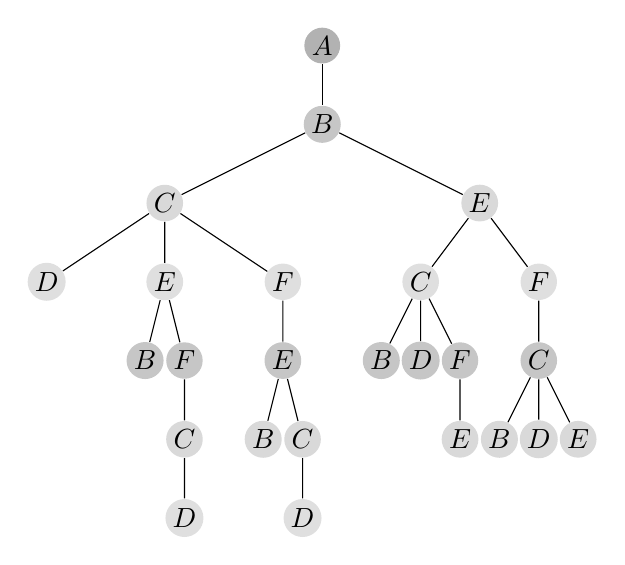
\begin{tikzpicture}
	[level distance=10mm,
	every node/.style={fill=gray!60,circle,inner sep=1pt},
	level 1/.style={sibling distance=20mm,nodes={fill=gray!45}},
	level 2/.style={sibling distance=40mm,nodes={fill=gray!30}},
	level 3/.style={sibling distance=15mm,nodes={fill=gray!25}},
	level 4/.style={sibling distance=5mm,nodes={fill=gray!45}},
	level 5/.style={sibling distance=5mm,nodes={fill=gray!30}},
	level 6/.style={sibling distance=5mm,nodes={fill=gray!25}},
	level 7/.style={sibling distance=5mm,nodes={fill=gray!45}}
	]
	\node {$A$}
		child {node{$B$}
			child {node{$C$}
				child {node{$D$}}
				child {node{$E$}
					child {node{$B$}}
					child {node{$F$}
						child {node{$C$}
							child {node{$D$}}
						}
					}
				}
				child {node{$F$}
					child {node{$E$}
						child {node{$B$}}
						child {node{$C$}
							child {node{$D$}}
						}	
					}
				}
			}
			child {node{$E$}
				child {node{$C$}
					child {node{$B$}}
					child {node{$D$}}
					child {node{$F$}
						child {node{$E$}}
					}
				}
				child {node{$F$}
					child {node{$C$}
						child {node{$B$}}
						child {node{$D$}}
						child {node{$E$}}
					}
				}
			}
		};
	\end{tikzpicture}
    \caption{Total de maneras en las que el hombre puede detenerse a almorzar.}
\end{figure}

\subsection{Problema 2.74}

Considere el diagrama adyacente con nueve puntos $A, B, C, R, S, T, X, Y, Z$.
Una persona comienza en $X$ y se le permite moverse horizontal o verticalmente,
un paso a la vez. Se detiene cuando no puede seguir caminando. sin llegar al
mismo punto más de una vez. Encuentra el número de maneras en que puede tomar su
caminata, si primero se mueve de $X$ a $R$. (Por simetría, el número total de
vías es el doble).

\begin{figure}[h!]
	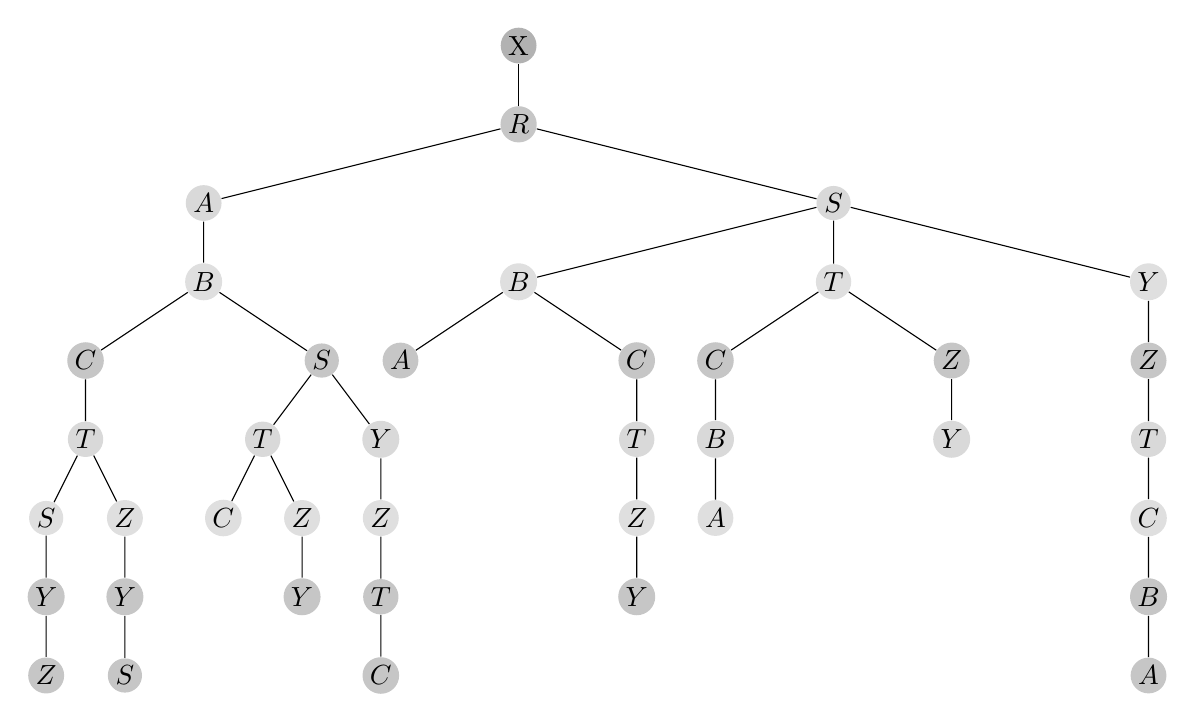
\begin{tikzpicture}
	[level distance=10mm,
	every node/.style={fill=gray!60,circle,inner sep=1pt},
	level 1/.style={sibling distance=20mm,nodes={fill=gray!45}},
	level 2/.style={sibling distance=80mm,nodes={fill=gray!30}},
	level 3/.style={sibling distance=40mm,nodes={fill=gray!25}},
	level 4/.style={sibling distance=30mm,nodes={fill=gray!45}},
	level 5/.style={sibling distance=15mm,nodes={fill=gray!30}},
	level 6/.style={sibling distance=10mm,nodes={fill=gray!25}},
	level 7/.style={sibling distance=5mm,nodes={fill=gray!45}}
	]
	\node {X}
		child {node{$R$}
			child {node{$A$}
				child {node{$B$}
					child {node{$C$}
						child {node{$T$}
							child {node{$S$}
								child {node{$Y$}
									child {node{$Z$}}
								}
							}
							child {node{$Z$}
								child {node{$Y$}
									child {node{$S$}}
								}
							}
						}
					}
					child {node{$S$}
						child {node{$T$}
							child {node{$C$}}
							child {node{$Z$}
								child {node{$Y$}}
							}
						}
						child {node{$Y$}
							child {node{$Z$}
								child {node{$T$}
									child {node{$C$}}
								}
							}
						}
					}
				}
			}
			child {node{$S$}
				child {node{$B$}
					child {node{$A$}}
					child {node{$C$}
						child {node{$T$}
							child {node{$Z$}
								child {node{$Y$}}
							}
						}	
					}
				}
				child {node{$T$}
					child {node{$C$}
						child {node{$B$}
							child {node{$A$}}
						}
					}
					child {node{$Z$}
						child {node{$Y$}}
					}
				}
				child {node{$Y$}
					child {node{$Z$}
						child {node{$T$}
							child {node{$C$}
								child {node{$B$}
									child {node{$A$}}
								}
							}
						}
					}
				}
			}
		};	
	\end{tikzpicture}
    \caption{Número de maneras en las que puede realizar su caminata.}
\end{figure}

% Set the overall layout of the tree
\tikzstyle{level 1}=[level distance=1.3cm, sibling distance=1cm]
\tikzstyle{level 2}=[level distance=2cm, sibling distance=7cm]
\tikzstyle{level 3}=[level distance=1.5cm, sibling distance=3cm]
\tikzstyle{level 4}=[level distance=1.5cm, sibling distance=2.5cm]
\tikzstyle{level 5}=[level distance=1.5cm, sibling distance=1cm]

% Define styles for bags and leafs
\tikzstyle{bag} = [text width=4em, text centered]
\tikzstyle{end} = [circle, minimum width=3pt,fill, inner sep=0pt]

\begin{figure}[h!]
\begin{tikzpicture}[grow=right, sloped]
    \node[bag] {X}
    child {
        node[bag] {R}
    child {
        node[bag] {S}
                                         child {
                    node[bag] {Y}
                                                     child {
                    node[bag] {Z}
                                                     child {
                    node[bag] {T}
                                                     child {
                    node[bag] {C}
                                                     child {
                    node[bag] {B}
                                                     child {
                    node[bag] {A}
                }
                }
                }
                }
                }
                }
                                                 child {
                    node[bag] {T}
                                                     child {
                    node[bag] {Z}
                                                     child {
                    node[bag] {Y}
                }
                }
                                                 child {
                    node[bag] {C}
                                                     child {
                    node[bag] {B}
                                                     child {
                    node[bag] {A}
                }
                }
                }
                }
        child {
                node[bag] {B}
                                                 child {
                    node[bag] {C}
                                                     child {
                    node[bag] {T}
                                                     child {
                    node[bag] {Z}
                                                     child {
                    node[bag] {Y}
                }
                }
                }
                }
                                                 child {
                    node[bag] {A}
                }
    }
    }
    child {
        node[bag] {A}
            child {
                node[bag] {B}
                            child {
                node[bag] {S}
                                                 child {
                    node[bag] {Y}
                                                     child {
                    node[bag] {Z}
                                                     child {
                    node[bag] {T}
                                                     child {
                    node[bag] {C}
                }
                }
                }
                }
                                                 child {
                    node[bag] {T}
                                                     child {
                    node[bag] {Z}
                                                     child {
                    node[bag] {Y}
                }
                }
                                                 child {
                    node[bag] {C}
                }
                }
            }
                            child {
                node[bag] {C}
                                 child {
                    node[bag] {T}
                                    child {
                    node[bag] {Z}
                                                     child {
                    node[bag] {Y}
                                                     child {
                    node[bag] {S}
                }
                }
                }
                                                 child {
                    node[bag] {S}
                                                     child {
                    node[bag] {Y}
                                                     child {
                    node[bag] {Z}
                }
                }
                }
                }
            }
            }
            }
    };
\end{tikzpicture}
\caption{Diagrama de árbol con las diferentes maneras en las que se puede tomar el camino}
\end{figure}

